\newpage
\section{Question 4}
	\noindent
	\newline
	We have used given 10 images in camera calibration tool provided. After the calibration it provides us details on following two major parameters:\newline
	
	\hspace{30} 1.	Intrinsic parameters(camera model)\newline
	
	\hspace{30} 2.	Extrinsic parameters\newline
	
	
	Under Intrinsic parameters it provided information about:\newline
	
	\hspace{30} 1. Focal length: The focal length in pixels - ${f_c}$\newline
	
	\hspace{30} 2. Principal point: The principle point coordinates – ${cc}$\newline
	
	\hspace{30} 3. Skew coefficient: The skew coefficient defining the angle between the ${x}$ and ${y}$ pixel axes - ${\alpha_c}$\newline
	
	\hspace{30} 4.	Distortions: The image distortion coefficients (radial and tangential distortions) - ${k_c}$\newline
	\newline
	(Reference: http://www.vision.caltech.edu/bouguetj/calib_doc/htmls/parameters.html)\newline
	\newline
	
	\subsection{Initial results after corner extraction}
	\newline
	Following are the calibration results after initial calibration with a Pixel error of ${[0.81041,   0.57619]}$.\newline
	\begin{figure}[position = here]
		\begin{centering}
			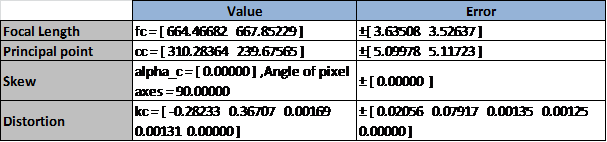
\includegraphics[scale=1.5]{q4_1}\\
		\end{centering}
	\end{figure}
	\newline
	\pagebreak
	\newline fter reprojecting above resulting calibration to the images following were the results. (1st two)\newline
	\begin{figure}[position = here]
		\begin{centering}
			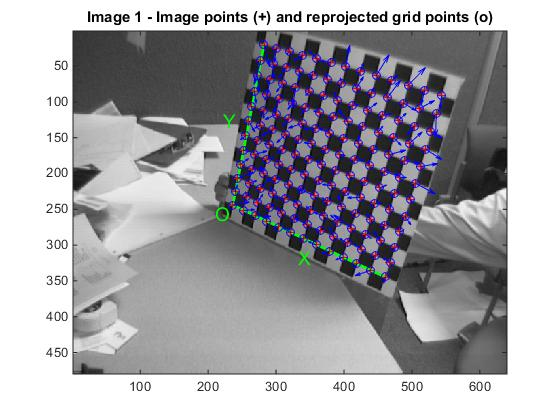
\includegraphics[scale=0.5]{q4_2}\\
		\end{centering}
	\end{figure}
	\newline
	\begin{figure}[position = here]
		\begin{centering}
			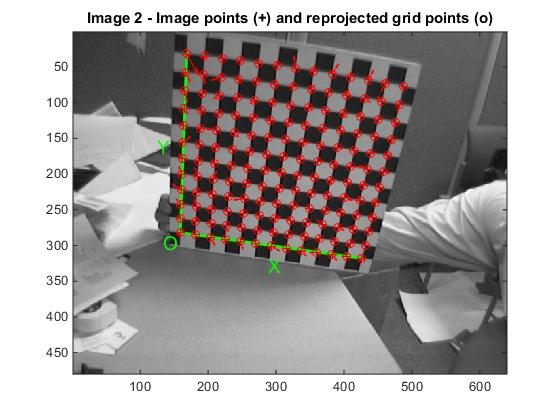
\includegraphics[scale=0.5]{q4_3}\\
		\end{centering}
	\end{figure}
	\newline
	The reprojection error for the initial calibration is as follows. (in the form of color-coded crosses)\newline
	\pagebreak
	
	
	\newline
	\begin{figure}[position = here]
		\begin{centering}
			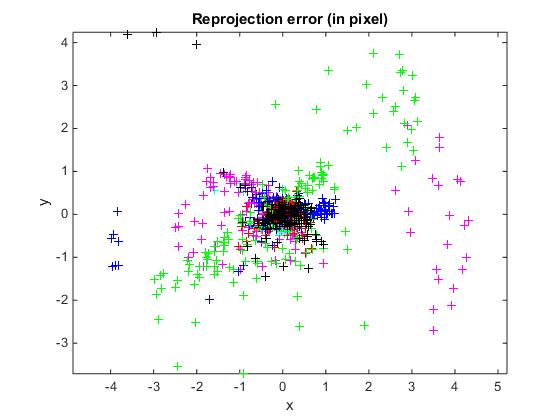
\includegraphics[scale=0.5]{q4_4}\\
		\end{centering}
	\end{figure}
	\newline
	
	We recompute the image corners on all images using the re-projected grid as initial guess locations for the corners to reduce the error automatically. This was done using Recomp. corners.  Then calibrate it again. This gives us improved results.\newline
	
	\pagebreak
	\subsection{Results after Final Calibration}
	\newline
	Calibration results after optimization after initial calibration:\newline
	\begin{figure}[position = here]
		\begin{centering}
			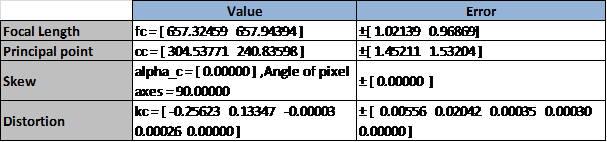
\includegraphics[scale=1.5]{q4_5}\\
		\end{centering}
	\end{figure}
	\newline
	After projecting final calibration results to the images, (1st two)\newline
	
	
	\begin{figure}[position = here]
		\begin{centering}
			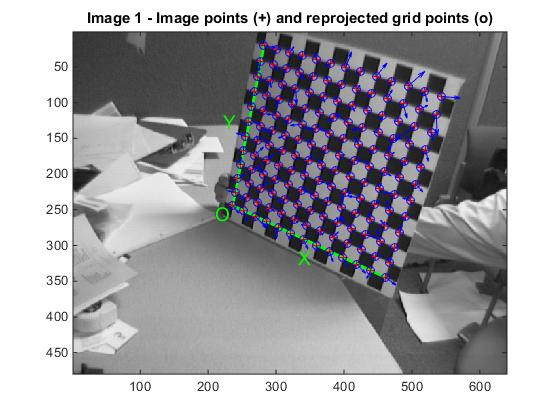
\includegraphics[scale=0.5]{q4_6}\\
		\end{centering}
	\end{figure}
	\newline
	\pagebreak
	\begin{figure}[position = here]
		\begin{centering}
			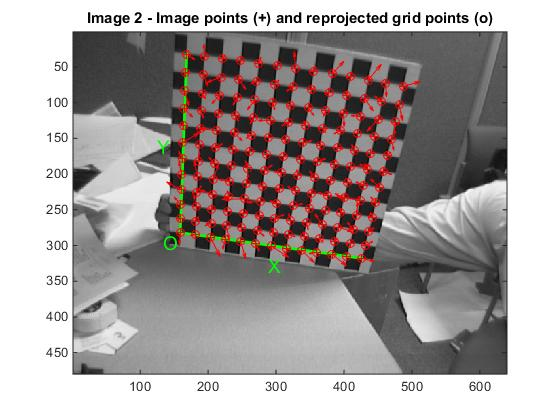
\includegraphics[scale=0.5]{q4_7}\\
		\end{centering}
	\end{figure}
	\newline
	We can’t see a much difference in these pictures by just looking at it. But in pixel level the error has reduced a lot.\newline \newline
	Reprojection error in final calibration:\newline
	
	
	\begin{figure}[position = here]
		\begin{centering}
			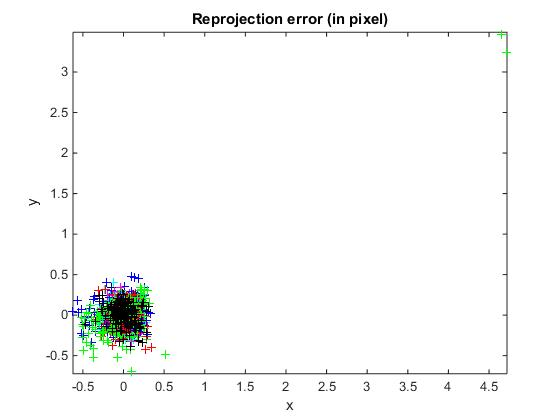
\includegraphics[scale=0.5]{q4_8}\\
		\end{centering}
	\end{figure}
	\newline
	
	\pagebreak
	



\pagebreak